\documentclass[12pt, titlepage]{article}
\usepackage{xcolor} % for different colour comments

%% Comments
\newif\ifcomments\commentstrue

\ifcomments
\newcommand{\authornote}[3]{\textcolor{#1}{[#3 ---#2]}}
\newcommand{\todo}[1]{\textcolor{red}{[TODO: #1]}}
\else
\newcommand{\authornote}[3]{}
\newcommand{\todo}[1]{}
\fi

\newcommand{\wss}[1]{\authornote{magenta}{SS}{#1}}
\newcommand{\ds}[1]{\authornote{blue}{DS}{#1}}

%% Graphics
\usepackage{float}
\usepackage{caption}
\usepackage{graphicx}
\graphicspath{ {Images/} }

\begin{document}

\title{ClinicFlow Software Requirments} 
\author{Maxim Vasiliev \#400043983 \\ Susie Yu \#000955758\\ Karl Knopf \#001437217 \\ Weilin Hu \#001150873 \\ Yunfeng Li \#001335650}
\date{\today}
\maketitle

\tableofcontents 

\listoffigures

\listoftables
\pagebreak

\begin{table}[H]
\section*{Revision History}
\begin{tabular}{|c|c|}
\hline
\textbf{Date}  & \textbf{Comments} \\ \hline
October 11, 2016 &  first draft. \\ 
\hline
\end{tabular}
\caption{Revision History Table}
\end{table}

\section*{Template}
This document uses Volere Template for its organization.
\pagebreak

\section{Changes made}
\begin{itemize}
 \item None
\end{itemize}

\section{Project Drivers}

\subsection{The Purpose of the Project}
This project aims to produce a tool which allows parties in the pre-operative clinic sector to optimize scheduling of patients amongst different procedures at the clinic, as well as arrival time and date to the clinic. Demand for the solution stems from the lack of relevant products, and the reliance of clinic staff on intuitive and error prone manual scheduling. With this tool, prior patient temporal data will be feed in and used to build a model of the variable involved. A simulation engine will then be used to produce an optimized scheduling of patients under inputted constraints. This would allow clinic staff to reduce scheduling errors, as well as conserve resources by automating the scheduling process.
\subsection{The Stakeholders}
\subsubsection{The Client}
Prospective clients of this product would include any clinics providing a set of different procedures, admitting patients to undergo some subset of those procedures, and who wish to automate their scheduling processes. Other potential clients include operators of any systems which make available a set of processes of different durations, which hope to automate scheduling of multiple concurrent uses of said services under various constraints.
\subsubsection{The Users}
Intended Users include employees of clinics or systems described above. In both cases, users are under time/resource constraint to perform their assigned scheduling functions.
\subsubsection{The Patients}
This group includes the individual components to be scheduled through the system. In the case of patients, this would concern individuals whose well-being and quality of service is of importance to themselves and their satisfaction of system performance.
\subsubsection{Other Stakeholders}
Other Stakeholders of this project include:
\begin{itemize}
  \item     Supervisors: Dr. Wenbo He, Dr. Douglas Down, Steve Metham
  \item 	Clinic manager
\end{itemize}

\section{Project Constraints}
\subsection{Mandated Constraints}
\subsubsection{Cost Constraints}
There is no immediate financial cost associated with project development. Clinic employees may have to devote some time for requirements gathering and product testing sessions. If however the system is successful and to be put in place permanently, use of a dedicated server will be required. For this, a cloud hosting and compute service such as Amazon Web Services would suffice. Financial cost for hosting and data access should be minimal, while compute costs will be determined during development, and dependant on algorithm performance.
\newline
\subsubsection{Quality Constraints}
One measure of project success is the quality of results. Since program output will be used in a live clinic environment, it is important that the proposed optimal schedule be verifiable in production. This requires that schedules be tested in situ, and performance compared to manually scheduled historical data. This proof is necessary to implement use of the product in field.
\newline\
\subsubsection{Risks}
Building on the quality considerations above, one evident risk would be failure of generated schedules to demonstrate improvements over control (previous method of scheduling). This may cause bottlenecks or backlogs in patients processing, placing additional stress on clinic employees and institution finances. 
\newline\
\subsubsection{Scheduled Deliverable and Development Time}
The final deadline for the project is mid April 2017. The detailed deliverable and their respective deadlines are listed below:
\begin{itemize}
  \item Requirements Document - revision 0: October 12, 2016 
  \item Proof of Concept Plan: October 26, 2016
  \item Test Plan - Revision 0: November 2, 2016
  \item Proof of Concept Demonstration: November 21, 2016
  \item Design Document - Revision 0: January, 11, 2016
  \item Demonstration - Revision 0: February 13, 2017
  \item User’s Guide - Revision 0: March 1, 2017
  \item Test Plan - Revision 0: March 22, 2017
  \item Final Demonstration: Mid-April, 2017
  \item Final Documentation: April 5, 2017
\end{itemize}

\subsection{Required resources}
\subsubsection{Available Data}
Historical patient arrival and procedure duration times will be provided by the client. These will be used to build the model for the variables such as deviation between patient scheduled and actual arrival times, and average and standard deviation of performed procedures.\newline\
Clinic constraints and business rules will also be provided by the client. This includes facts such as the number and shift of clinic employees, as well as rules such and allotted break times and intended shift end times for specific employees.
\newline\

\subsection{Relevant Facts and Assumptions} 
\subsubsection{Relevant Facts}
N/A 
\newline
\subsubsection{Assumptions}
N/A

\section{Functional Requirements} 
\subsection{The Scope of the Product}
A desktop application or web-interface application can allow users to insert necessary data, such historical patient procedure durations, doctor and nurse shift hours, and other constraints such as break allotments or soft constraints such as employee shift end times. Based on provided data and inputs, the system will generate patient schedules for both arrival time into the clinic, and between procedures within the clinic. This tool will be designed with the intention to be implementable in multiple health care institutions for automating and managing patient scheduling
\subsubsection{Product Boundary}
Users gather the information from patients, doctors and clinic departments as input into the application, and receive schedules as outputs from the application. The inputs include historical patient data (arrival time, procedure time, departure time), doctor work hours, and other constraints. The application stores the inputs into a database, and extracts the data when generating schedules. The schedule generator uses this data to produce schedules, and stores them into the database to be recalled at a later point. Users can update the database and adjust schedules at any time, rerunning the simulation engine to produce an updated prediction of daily clinic flow statistics.

\begin{figure}[H]
  \centering
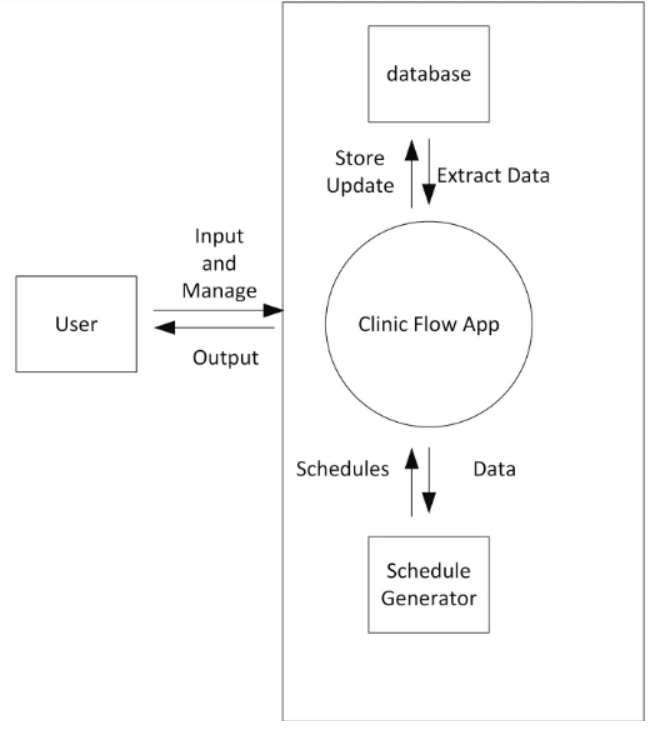
\includegraphics[scale=0.9]{product_boundary.png}
\caption{Product Boundary Diagram}
\end{figure}

\subsubsection{Product Use Case Table}
\begin{center}
\begin{table}[H]
  \centering
\begin{tabular}{ |c|c|c|c| }
\hline
PUC\# & PUC Name & Actors & Summary \\
\hline
1 & Login & User & Access the application \\
2 & Insert Information & User & Insert information of patients and doctors \\
3 & Store Information & User & Save the entered data to database \\
4 & Display Data & User & View the data \\
5 & Update Data & User & Changer the data inside database \\
6 & Generate Schedules & User & Assign patients to procedure slots \\
7 & Store Schedules & User & Save generated schedules into database \\
8 & Display Schedules & User & View existed schedules \\
9 & Adjust Schedules & User & Change the existed schedules \\
10 & Log out & User & Leave the system and close the authority  \\
\hline
\end{tabular}
\caption{Use Case Table}
\end{table}
\end{center}

\subsection{Functional Requirements}
\textbf{\textit{Requirement 1}}\newline
\textit{Description:}\newline
The product shall verify the user’s authority to access the full system.\newline\newline
\textit{Fit Criterion:}\newline 
The product should require user to pass one or more security guards before the user start managing the system. 
\newline

\noindent\textbf{\textit{Requirement 2}}\newline
\textit{Description:}\newline
The product shall allow the user to enter data.\newline\newline
\textit{Fit Criterion:}\newline 
Users can enter any type of data into the system such as strings, integers and datetimes. Then the application must send the inputted data to the database.
\newline

\noindent\textbf{\textit{Requirement 3}}\newline
\textit{Description:}\newline
The product shall allow the user to manage the information in the database. \newline\newline
\textit{Fit Criterion:}\newline 
Users can update and modify the data inside database at any moment. Users can create more data types or tables for dealing with changes in the future.
\newline

\noindent\textbf{\textit{Requirement 4}}\newline
\textit{Description:}\newline
The product shall match the available time of patients and doctors to generate an optimal schedule. \newline\newline
\textit{Fit Criterion:}\newline 
The product extracts information from database, and match time table of doctors with the available time of patients. Base on an algorithm, the product can generate schedules based on a first in first out query or create schedules for all patients as a pooled schedule. The generated schedules will be stored into the database. \newline

\noindent\textbf{\textit{Requirement 5}}\newline
\textit{Description:}\newline
The product shall be able to show the data inside database to user in an informative way. \newline\newline
\textit{Fit Criterion:}\newline 
Users can open and view details of all data inside database. The data includes the information from patients, information from doctors, and previously generated schedules. \newline

\noindent\textbf{\textit{Requirement 6}}\newline
\textit{Description:}\newline
The product shall allow users to adjust generated schedules. \newline\newline
\textit{Fit Criterion:}\newline 
The user can adjust the previously generated schedules by changing the time of the schedules. The user can update the available times of patients or doctors, and regenerate schedules. \newline

\noindent\textbf{\textit{Requirement 7}}\newline
\textit{Description:}\newline
The product shall alert the user of any time conflicts between patients and doctors. \newline\newline
\textit{Fit Criterion:}\newline 
The product should monitor the process of generating schedule and adjusting schedules.When a insolvable conflict appears, they product should remind the user that such conflicts exist. \newline

\noindent\textbf{\textit{Requirement 8}}\newline
\textit{Description:}\newline
The product shall provide the most optimized schedules to the users first. \newline\newline
\textit{Fit Criterion:}\newline 
The product must consider the  arrival time, waiting time, service time of different procedure for a patient in clinic. The product should try to minimize the total time patients spend in the clinic. Meanwhile, the product should minimize the idle time of doctors. \newline

\section{Nonfunctional Requirements}
\subsection{Look and Feel Requirements}
\textit{Description:}\newline
The user interface for this application will be clean in design. It will provide simple menus from which the user can select desired tasks. There will be a window to view the output, and an attached menu with options to save the results. 
\newline \newline 
\textit{Fit Criterion:}\newline 
The application should have no unnecessary windows and menus.
The application should generate no complaints from users about being unable to find a specific option.
\subsection{Usability Requirements}
\subsubsection{Ease of Use Requirements}
\textit{Description:}\newline
Intended users include managers of preoperative clinics, or other organizations with similar scheduling goals. While these parties may not be experienced using complex software and non-graphical user interfaces, it is assumed they have some experience using common software products. As such, the program interface and output should be intuitive and readily interpretable
\newline \newline 
\textit{Fit Criterion:}\newline 
The application interface should be graphical.
Program output should be presented and formatted in a manner which quickly and clearly conveys pertinent information, as well as being able to be shared and distributed amongst clinic staff.
\subsubsection{Language Requirements}
\textit{Description:}\newline
The application should be written in and provide feedback in Canadian English. Future version may may support for other languages.
\newline \newline 
\textit{Fit Criterion:}\newline 
Only Canadian English will be used in the graphic interface and outputs.
Design the software so that the language may be eventually changed.

\subsection{Performance Requirements}
\subsubsection{Speed and Latency Requirements}
\textit{Description:}\newline
The program should respond quickly to user input. The application should run the simulation in reasonable time, given the data size.
\newline \newline 
\textit{Fit Criterion:}\newline 
Interactions between user and system shall have a maximum response time of 2 seconds. Each simulation should take between 30 seconds and 30 minutes (guesses), depending on the data size.

\subsubsection{Reliability and Availability Requirements}
\textit{Description:}\newline
The product shall be available for use 24 hours per day, 365 days per year.
\newline \newline 
\textit{Fit Criterion:}\newline 
The product should not need any downtime to function. If the system is web based, then it should have 99\% up time.

\subsubsection{Scalability or Extensibility Requirements}
\textit{Description:}\newline
The product should be able to handle the initial data set, around 900 data points but it should be able to scale to at least 10000 data points as the data set grows.
\newline \newline 
\textit{Fit Criterion:}\newline 
The simulation engine of the program should not be bound by the size of the data. The application should be able to save the necessary data in an accessible format.

\subsubsection{Robustness or Fault Tolerance Requirements}
\textit{Description:}\newline
The program should prompt the user if it is unable to run the simulation on the first try. As well if the user tries to run an operation and it fails, the user should be notified. 
\newline \newline 
\textit{Fit Criterion:}\newline 
A warning message will be provided to the user if the simulation is unable to be run.
A warning message will be provided to the user if their selected operation can be be done.

\subsection{Maintainability and Support Requirements}
\subsubsection{Maintenance Requirements}
\textit{Description:}\newline
Changes to system will be done within one week of being presented to the maintenance team. Changes will be applied to the application as soon as they are available.
\newline \newline 
\textit{Fit Criterion:}\newline 
There is only a delay of a week between the report of an error in the software, and a fix being applied. There is no downtime between the creation of a fix and its application to the program.

\subsubsection{Supportability Requirements}
\textit{Description:}\newline
The user of the software should have direct access to the support team, and be able to make a request directly to the team.
\newline \newline 
\textit{Fit Criterion:}\newline 
A system to allow the client to report directly to the team shall be implemented.

\subsubsection{Adaptability Requirements}
\textit{Description:}\newline
As the application will be web-based, it should be accessible from any operating system that has internet browsing capability. Furthermore, if needed the application can be made to run locally on some machine by installing all server components on said machine.
\newline \newline 
\textit{Fit Criterion:}\newline 
The application runs on Amazon Web Services. Adaptability to other systems should be considered during system design.

\subsection{Security Requirements}
\subsubsection{Access Environment}
\textit{Description:}\newline
Managers of the clinic posses full administrative access to the program. Doctors and nurses may be able to see historical results of simulations but may not run them.
\newline \newline 
\textit{Fit Criterion:}\newline 
The program should have two sets of credentials granting access to it. Credentials consist of a username and a password. One set grants access to full administrative level program functions, while the other allows only observational access. 

\subsubsection{Privacy Requirements}
\textit{Description:}\newline
The system should not store any personal information, and the data should be clean of any personal information before being entered. The output should use generic names (Nurse 1) to create a schedule, the assignment of the generic names to actual people is left up to the manager.
\newline \newline 
\textit{Fit Criterion:}\newline 
Historical patient data used to build the model will have all personally identifiable information removed prior to being handed to the development team. The application is unable to save personal information. The application does not use specific names when creating a schedule.

\section{Project Issues}
\subsection{Design Decisions}
The implementation and working environment dependencies:
\begin{itemize}
  \item HTML, CSS and JavaScript will be used to write the graphical user interface.
  \item PHP will be used as an interface to the database due to its simplicity
  \item MongoDB will also be used due to its simplicity and non-essentiality of a relational model for data storage. 
  \item The simulation and optimization engine will be written in Python. Specifically, the SimPy package will be used for discrete event simulation components.
  \item The application can be installed locally on a computer, or it can be  
  	accessed from a remote server.
\end{itemize}

\subsection{Off the Shelf Solutions}
\subsubsection{Ready Made Products}
There are many commercial scheduling software existing in the market, however, they do not offer scheduling optimization and patient flow simulation functions.

\subsubsection{Reusable Components}
Because the source code of commercial software is not available, there is no reusable component.

\subsection{Costs}
The product will be open-source, but if it is installed on a server, maintenance fees and Internet fee may apply.

\subsection{Alternative Ideas}
The current protocol for scheduling involves patients being immediately given a time to arrive at the clinic. This sets the system up for inefficiencies because the total set of patients to be scheduled are not known ahead of time. The potential therefore exists to implement a scheduling protocol whereby patients are placed into a pool instead of immediately being given an appointment time. Once the pool reaches a threshold, all patients in the pool are scheduled together. This allow the system to make a far more optimal daily schedule since all patients to be scheduled are known ahead of time. Performance of this alternative scheduling method can be compared to the current method using both the presently proposed tool, as well as in production.

\end{document}